\item \textbf{{[}DHS/PRELIM/9597/2014/P2/Q2{]} }

The following invoice shows the medical bill incurred by a pioneer
in a polyclinic. 
\begin{center}
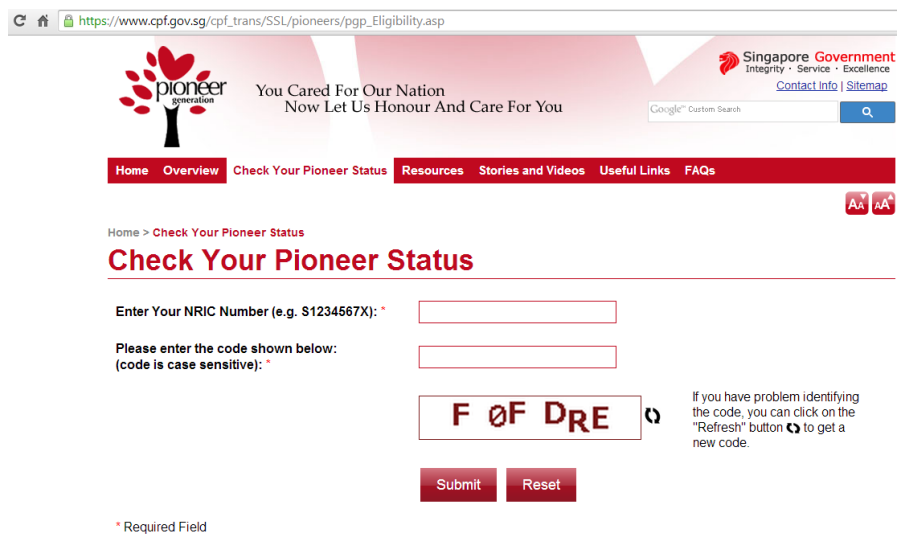
\includegraphics[width=0.65\paperwidth]{C:/Users/Admin/Desktop/Github/question_bank/LyX/static/img/9597-DHS-2014-P1-Q1}
\par\end{center}

A normalised database solution is to be designed, which has a number
of tables.
\begin{enumerate}
\item Derive the normalised process from the unnormalised form (UNF) to
the third normal form (3NF). \hfill{}{[}7{]}
\item Draw an ER diagram that shows these tables and the relationships between
them. \hfill{}{[}3{]}
\item Using suitable examples, explain the concepts of 
\begin{enumerate}
\item primary key \hfill{}{[}1{]}
\item foreign key \hfill{}{[}2{]}
\item composite key \hfill{}{[}2{]}
\end{enumerate}
\end{enumerate}